% methodology.tex --- Section 3
% Contains the full Voting Ensemble Paradox proof (stated constraint) and the
% asymmetric loss modulation derivation. Architecture subsection is outlined
% pending the remaining sections.
\section{Methodology}
\label{sec:methodology}

\subsection{Setup and notation}
\label{sec:setup}

Let $X$ be the space of tokens (or segments) subject to pruning. We partition
$X$ into $K$ disjoint \emph{strata} $S_1,\dots,S_K$ by syntactic role
(e.g., identifier, path literal, exit code, delimiter, prose). Let
$V_1,\dots,V_N$ be $N$ compression checkpoints with asymmetric
\textbf{training-data floors} $f_1 \le f_2 \le \dots \le f_N$, where lower $f_i$
denotes a weaker training condition (less data or noisier silver labels).
Let $\I_i(x) \in \{0,1\}$ be the \emph{eviction indicator} for voter $V_i$:
$\I_i(x)=1$ iff $V_i$ evicts $x$. Denote the rejection set
$R_i = \{x : \I_i(x)=1\}$. Let $K^{\star}\subseteq X$ be the ground-truth
keep set (true-keep tokens).

\begin{definition}[Asymmetric data floor]
\label{def:floor}
A checkpoint $V_i$ has training-data floor $f_i$, drawn from an ordered set
$F=\{f_1\le\dots\le f_N\}$ with at least two distinct levels ($f_1 < f_N$).
Lower floors correspond to weaker training conditions and, empirically, to
larger rejection sets on the strata those conditions under-represent.
\end{definition}

\begin{definition}[Per-stratum monotone-rejection refinement]
\label{def:monotone}
The voter pool satisfies \emph{per-stratum monotone-rejection refinement} if
for every stratum $S_k$ there exists a voter $i^{\star}_k \in [N]$---the
\emph{weakest voter on $S_k$}---such that for all $i \in [N]$ and all
$x \in S_k$,
\[
  \I_{i^{\star}_k}(x) \;\ge\; \I_i(x).
\]
Equivalently, $R_{i^{\star}_k} \cap S_k \supseteq R_i \cap S_k$ for all $i$:
on stratum $S_k$ the weakest voter rejects a superset of every other voter's
rejections.
\end{definition}

\begin{remark}[Empirical status of Definition~\ref{def:monotone}]
Definition~\ref{def:monotone} is a sufficient condition, not a necessary one.
In practice, voters disagree in non-nested ways: two checkpoints may each
evict tokens the other keeps on the same stratum. The ensemble collapse we
observe (Section~\ref{sec:eval:paradox}) is consistent with, but does not
strictly require, Definition~\ref{def:monotone} holding exactly. We
\emph{assume} it as a modeling simplification that yields a clean closed-form
(Theorem~\ref{thm:paradox}); the empirical $0.961\to0.931$ regression
demonstrates that \emph{some} form of per-stratum weakest-voter dominance
is present in the v3/v4/v5 ensemble, even if the strict inclusion
$R_{i^{\star}_k}\cap S_k \supseteq R_i\cap S_k$ does not hold for every
token. A full empirical verification (per-stratum rejection-set inclusion
matrices) is left to future work with larger eval sets.
\end{remark}

This encodes the empirical observation that a checkpoint trained on a lower
floor over-evicts on the strata its training data under-represented, while a
higher-floor checkpoint is more selective on those same strata. Crucially, the
identity of the weakest voter may differ across strata.

\begin{definition}[Unanimity-to-keep (AND) ensemble]
\label{def:and}
The ensemble $\hat V$ evicts $x$ iff at least one voter evicts:
\[
  \I_{\mathrm{ens}}(x)
  \;=\; \bigvee_{i=1}^{N} \I_i(x)
  \;=\; 1 - \prod_{i=1}^{N}\bigl(1-\I_i(x)\bigr).
\]
A token is kept iff \emph{all} voters agree to keep it.
\end{definition}

\begin{definition}[$k$-of-$N$ drop ensemble]
\label{def:kofn}
For drop threshold $k_{\mathrm{drop}}\in\{1,\dots,N\}$ (abbreviated $k$), the
$k$-of-$N$ drop ensemble evicts $x$ iff at least $k$ voters evict:
\[
  \I_{\mathrm{ens}}^{(k)}(x)
  \;=\; \mathbf{1}\!\left[\textstyle\sum_{i=1}^{N} \I_i(x) \;\ge\; k\right],
\]
where $\mathbf{1}[\cdot]\in\{0,1\}$ denotes the indicator function. Equivalently,
a token is kept iff at least $k_{\mathrm{keep}} = N - k + 1$ voters vote to
keep it. Thus unanimity-to-keep (AND-keep / drop-if-any, Definition~\ref{def:and})
is $k{=}1$ ($k_{\mathrm{keep}}{=}N$); majority of $3$ is $k{=}2$
($k_{\mathrm{keep}}{=}2$); and unanimity-to-drop (OR-keep / keep-if-any) is
$k{=}N$ ($k_{\mathrm{keep}}{=}1$).
\end{definition}

\subsection{The Voting Ensemble Paradox}
\label{sec:paradox}

\begin{theorem}[Voting Ensemble Paradox]
\label{thm:paradox}
Under unanimity-to-keep voting (Definition~\ref{def:and}, $k{=}1$), for every
stratum $S_k$ and any arbitrary voter pool $\{V_1,\dots,V_N\}$, the false-eviction
rate on ground-truth keep tokens $S_k \cap K^{\star}$ is bounded below by the
worst voter on that stratum:
\[
  \Pr\!\bigl[\I_{\mathrm{ens}}(x)=1 \;\big|\; x\in S_k\cap K^{\star}\bigr]
  \;\ge\;
  \max_{i\in[N]}\;\Pr\!\bigl[\I_i(x)=1 \;\big|\; x\in S_k\cap K^{\star}\bigr].
\]
Moreover, under per-stratum monotone-rejection refinement
(Definition~\ref{def:monotone}), for every $x \in S_k$,
\[
  \I_{\mathrm{ens}}(x) \;=\; \I_{i^{\star}_k}(x),
  \qquad\text{and}\qquad
  \Pr\!\bigl[\I_{\mathrm{ens}}(x)=1 \;\big|\; x\in S_k\cap K^{\star}\bigr]
  \;=\;
  \Pr\!\bigl[\I_{i^{\star}_k}(x)=1 \;\big|\; x\in S_k\cap K^{\star}\bigr].
\]
\end{theorem}

\begin{proof}
Fix a stratum $S_k$ and a token $x \in S_k$. Because each $\I_i(x)\in\{0,1\}$,
Definition~\ref{def:and} gives
$\I_{\mathrm{ens}}(x) = \bigvee_{i=1}^{N}\I_i(x) = \max_{i\in[N]}\I_i(x) \ge \I_j(x)$
for every $j\in[N]$. Taking conditional expectations over $x\in S_k\cap K^{\star}$
and maximizing over $j\in[N]$ yields the general distribution-free inequality
(which is strict whenever two voters make non-nested false evictions on
$S_k\cap K^{\star}$). Under Definition~\ref{def:monotone},
$\I_{i^{\star}_k}(x) \ge \I_i(x)$ for all $i\in[N]$, so
\[
  \I_{\mathrm{ens}}(x)
  \;=\; \max_{i\in[N]} \I_i(x)
  \;=\; \I_{i^{\star}_k}(x),
\]
and conditioning on $x \in S_k \cap K^{\star}$ gives the exact equality.
\end{proof}

\begin{corollary}[Stratum-wise recall collapse]
\label{cor:pareto}
Define per-stratum must-keep survival (keep-recall on $K^{\star}$) for voter $V$
as $\mathrm{Recall}_{S_k}(V) = \Pr[\I_V(x)=0 \mid x\in S_k\cap K^{\star}]$ and
stratum weights $w_k = \Pr[x\in S_k \mid x\in K^{\star}] = |S_k\cap K^{\star}|/|K^{\star}|$.
Under the conditions of Theorem~\ref{thm:paradox}, for each stratum $S_k$ the
ensemble's must-keep recall equals that of the weakest voter $V_{i^{\star}_k}$:
\[
  \mathrm{Recall}_{S_k}(\hat V)=\mathrm{Recall}_{S_k}(V_{i^{\star}_k}),
  \qquad\text{and}\qquad
  \mathrm{Recall}(\hat V)
  \;=\; \sum_{k=1}^{K} w_k\,\mathrm{Recall}_{S_k}(V_{i^{\star}_k})
  \;\le\; \min_{j\in[N]} \mathrm{Recall}(V_j),
\]
with strict inequality $\mathrm{Recall}(\hat V) < \max_{j\in[N]}\mathrm{Recall}(V_j)$
whenever the weakest voter differs across strata ($i^{\star}_k \neq i^{\star}_{k'}$
with strict floor gap on $S_k\cap K^{\star}$). Whenever $i^{\star}_k \neq i^{\star}_{k'}$
for some $k,k'$, the per-stratum recall vector
$\bigl(\mathrm{Recall}_{S_1}(\hat V),\dots,\mathrm{Recall}_{S_K}(\hat V)\bigr)$
is realized by no individual checkpoint and is component-wise dominated by any
single strong voter $V_j$. In the
$\bigl(\text{compression}=1-\mathit{keep\_rate},\;\text{must-keep recall}=\mathrm{Recall}\bigr)$
plane, $\hat V$ is Pareto-dominated by the threshold-swept frontier of a
single strong voter $V_j$ whenever $V_j$'s continuous score distribution separates
$K^{\star}$ from $X\setminus K^{\star}$ more cleanly on the strata where $j\neq i^{\star}_k$.
\end{corollary}

\begin{proof}
On each stratum $S_k$, $\mathrm{Recall}_{S_k}(\hat V) = 1 - \Pr[\I_{\mathrm{ens}}(x)=1 \mid x\in S_k\cap K^{\star}]
= 1 - \Pr[\I_{i^{\star}_k}(x)=1 \mid x\in S_k\cap K^{\star}] = \mathrm{Recall}_{S_k}(V_{i^{\star}_k})$
by Theorem~\ref{thm:paradox}. By the law of total probability over the disjoint
partition $\{S_k\cap K^{\star}\}_{k=1}^{K}$ of $K^{\star}$, global must-keep
recall is the linear combination $\mathrm{Recall}(V) = \sum_{k=1}^{K} w_k\,\mathrm{Recall}_{S_k}(V)$.
Because $\mathrm{Recall}_{S_k}(V_{i^{\star}_k}) \le \mathrm{Recall}_{S_k}(V_j)$
for every $j\in[N]$ and every $k$, summing with non-negative weights $w_k$
yields $\mathrm{Recall}(\hat V) \le \mathrm{Recall}(V_j)$ for every $j\in[N]$
(and strict inequality for any $V_j$ that strictly improves on $V_{i^{\star}_k}$
on at least one stratum with $w_k > 0$). Finally, if $i^{\star}_k \neq i^{\star}_{k'}$
with strict inclusions on $S_k\cap K^{\star}$ and $S_{k'}\cap K^{\star}$, no single
voter $V_j$ can simultaneously attain the minimum recall on both $S_k$ and $S_{k'}$.
\end{proof}

\paragraph{Interpretation.}
AND-keep ($k{=}1$) voting does not average voter competence; it takes, per
stratum, the \emph{most aggressive} eviction decision. Under asymmetric floors
this is the worst voter on that stratum. The ensemble is therefore a
Frankenstein of per-stratum worst cases---precisely the failure that motivates
the three correctives below.

\begin{remark}[$k$-of-$N$ generalization]
\label{rem:kofn}
Suppose that on each stratum $S_k$ the voters satisfy a nested chain of
rejection inclusions
$R_{\pi_k(1)}\cap S_k \supseteq R_{\pi_k(2)}\cap S_k \supseteq \dots \supseteq R_{\pi_k(N)}\cap S_k$
for some stratum-specific permutation $\pi_k$ ordering voters from weakest
($\pi_k(1)=i^{\star}_k$) to strongest ($\pi_k(N)$). Then the $k$-of-$N$ drop
ensemble (Definition~\ref{def:kofn}) evicts $x\in S_k$ iff the $k$-th largest
indicator on $S_k$ is $1$, i.e.\ $\I_{\mathrm{ens}}^{(k)}(x) = \I_{\pi_k(k)}(x)$
(the per-stratum $k$-th weakest voter). For AND-keep ($k{=}1$) this is the
weakest voter $\pi_k(1)$ (Theorem~\ref{thm:paradox}); for majority of $3$
($k{=}2$) it is the per-stratum \emph{median} $\pi_k(2)$; for unanimity-to-drop
(OR-keep, $k{=}N$) it is the strongest voter $\pi_k(N)$. Consequently, for every
$k < N$, $\mathrm{Recall}_{S_k}(\hat V^{(k)}) = \mathrm{Recall}_{S_k}(V_{\pi_k(k)})$,
which is dominated on stratum $S_k$ by any single voter $V_j$ whose per-stratum
rank is strictly stronger than $k$ ($\pi_k^{-1}(j) > k$). Our empirical
ensemble (Section~\ref{sec:eval:paradox}) evaluates both $k{=}2$ (majority) and
$k{=}1$ (drop-if-any) for $N{=}3$ and confirms the collapse.
\end{remark}

Figure~\ref{fig:paradox} illustrates the paradox: three checkpoints with
individual heretic scores of $0.942$, $0.967$, and $0.961$ combine under
majority voting to produce an ensemble score of $0.931$---worse than any
single model.

\begin{figure}[t]
  \centering
  \includegraphics[width=0.85\textwidth]{fig-paradox.pdf}
  \caption{The Voting Ensemble Paradox. Three checkpoints (v3, v4, v5) with
  individual heretic scores above $0.94$ combine under $k$-of-$N$ voting to
  produce an ensemble ($0.931$) that is Pareto-dominated by the best single
  model (v4, $0.967$). The collapse is stratum-dependent: each checkpoint is
  weakest on different token classes.}
  \label{fig:paradox}
\end{figure}

\subsection{Mechanism A: asymmetric loss modulation ($3.0\times$ penalty)}
\label{sec:loss}

Let $T_{\mathrm{crit}} \subset K^{\star} \subset X$ be the critical-syntactic
token class (signal names, file paths, exit codes, delimiters) identified by
the regex-driven must-keep thresholds of the ultrawhale-dogfood corpus. At
inference time, a false eviction on $T_{\mathrm{crit}}$ is captured by the
discrete indicator
$\I^{\mathrm{fe}}_i(x) = \I_i(x)\,\mathbf{1}[x \in T_{\mathrm{crit}}]$. To make
this penalty differentiable during training, let
$\ell_{\mathrm{ce}}(x;\theta_i) = -\bigl[y(x)\log p_{\theta_i}(\text{keep}\mid x)
+ (1-y(x))\log\bigl(1-p_{\theta_i}(\text{keep}\mid x)\bigr)\bigr]$ denote the
per-token cross-entropy against the binary keep label $y(x)\in\{0,1\}$. The
modulated token-classification loss $\mathcal{L}_{\mathrm{token}}(\theta_i)$
assigns multiplicative weight $\lambda = 3.0$ to critical tokens
($w(x) = 1 + (\lambda - 1)\,\mathbf{1}[x \in T_{\mathrm{crit}}]$):
\[
  \mathcal{L}_{\mathrm{token}}(\theta_i)
  \;=\;
  \frac{1}{|X|}\sum_{x\in X} w(x)\,\ell_{\mathrm{ce}}(x;\theta_i)
  \;=\;
  \underbrace{\frac{1}{|X|}\sum_{x\in X} \ell_{\mathrm{ce}}(x;\theta_i)}_{\Lbase(\theta_i)}
  \;+\;
  (\lambda - 1)\cdot
  \underbrace{\frac{1}{|X|}\sum_{x \in T_{\mathrm{crit}}}
              \bigl(-\log p_{\theta_i}(\text{keep}\mid x)\bigr)}_{\Lcrit(\theta_i)},
  \qquad \lambda = 3.0.
\]
$\Lcrit$ penalizes false-eviction log-loss on \emph{protected} tokens only
(since $y(x)=1$ for all $x\in T_{\mathrm{crit}}$). Although
the penalty is stratum-agnostic in its definition, false evictions concentrate
on each voter's weakest strata (where its training floor induced
over-eviction), so the gradient of $\Lcrit$ concentrates there as well. The
net effect is to shrink $|R_i \cap S_k|$ fastest for the voter that is
$i^{\star}_k$ on each stratum, lifting every per-stratum floor and raising the
collapse point of Corollary~\ref{cor:pareto} uniformly. We fix $\lambda=3.0$
for the production model (v8)---the empirically validated Pareto-optimal
point (Section~\ref{sec:eval:pareto}). The full ablation
$\lambda\in\{3,5,10\}$ maps a monotonic recall--compression frontier:
$\lambda{=}3$ yields $0.955$ heretic at $15\%$ compression (v8, production),
$\lambda{=}5$ yields $0.963$ at $3.7\%$ (v17), $\lambda{=}10$ yields $0.972$
at $2.8\%$ (v16, highest recall but near-zero compression).

\subsection{Dual-head architecture and the modulation gate}
\label{sec:arch}

\paragraph{Backbone.} kompress-v8 builds on the 149M-parameter dual-head
ModernBERT \citep{warner2024modernbert} architecture of
\texttt{chopratejas/kompress-v2-base}. The model lineage is
\texttt{answerdotai/ModernBERT-base} $\to$
\texttt{chopratejas/kompress-v2-base} $\to$ \texttt{PeetPedro/kompress-v8}.
The \texttt{v2-base} checkpoint provides the pretrained dual-head structure and
initial compression prior; our fine-tuning shifts the heads' salience toward
agent-critical tokens via mechanisms~A--C.

\begin{itemize}
  \item \textbf{Token-classifier head} $h_{\mathrm{tok}}$: linear projection
        producing per-token eviction logits $\mathrm{logit}_{\mathrm{tok}}(x)$,
        thresholded at $\tau=0.5$ to yield $\I_i(x)\in\{0,1\}$ at inference
        (while $p_{\theta_i}(\text{keep}\mid x) = 1 - \tilde{\I}_i(x)$).
  \item \textbf{Span-CNN head} $h_{\mathrm{span}}$: a 1D convolutional head
        (kernel width $k_{\mathrm{cnn}}{=}3$) over token windows that predicts
        span-level keep-coherence $\mathrm{logit}_{\mathrm{span}}(x)$ against
        the keep mask ($y(x)=1$), enforcing that evictions do not fragment
        protected syntactic units.
\end{itemize}

\paragraph{Asymmetric modulation gate.} The two heads are coupled by a
non-negative gate $g(z) = \mathrm{ReLU}(z)$ (with scale $\gamma > 0$) that
reduces the token-head eviction logit whenever the span head signals high
keep-coherence:
\[
  \tilde{\I}_i(x)
  \;=\;
  \sigma\!\bigl(\mathrm{logit}_{\mathrm{tok}}(x)
                - \gamma\, g\bigl(\mathrm{logit}_{\mathrm{span}}(x)\bigr)\bigr),
\]
where $\gamma > 0$ controls how strongly span-level \emph{keep-coherence}
suppresses per-token eviction. Because $g(z)\ge 0$ everywhere, the gate is
\emph{asymmetric}: it can only \emph{inhibit} eviction of tokens within
high-coherence keep spans, never promote eviction when
$\mathrm{logit}_{\mathrm{span}}(x) < 0$, which preserves the protected-token
guarantee that $\Lcrit$ relies on.

\subsection{Mechanism B: post-inference regex override}
\label{sec:override}

Mechanism~A reduces false evictions at training time but cannot eliminate
them: the $3.0\times$ penalty is a soft signal, and subword tokenization can
fragment multi-token must-keep patterns (e.g., \texttt{-O2} splits into
\texttt{-}, \texttt{O}, \texttt{2}). Mechanism~B is a \emph{surgical}
deterministic safety net applied after the model scores each token. Let
$\mathit{MUST\_KEEP\_RE}$ be the regex over decoded text matching the
critical-syntactic class (numbers, ALLCAPS identifiers, dotted paths, file
extensions, CLI flags, CamelCase, hex addresses). For each token position $t$
that the model would evict ($\I_i(x_t)=1$), contiguous windows
$W = (x_a,\dots,x_b)$ of length $1 \le b-a+1 \le 3$ containing $t$ ($a \le t \le b$)
are decoded and checked against $\mathit{MUST\_KEEP\_RE}$; if any such window
matches a critical span (without spanning whitespace into adjacent prose words),
every token $x_t$ in the matching span is force-kept:
\[
  \I^{(B)}_i(x_t)
  \;=\;
  \I_i(x_t)\,\wedge\,\bigwedge_{\substack{W=(x_a,\dots,x_b)\\ a\le t\le b,\; 1\le |W|\le 3}}
  \neg\,\mathrm{Match}_{\mathit{MUST\_KEEP\_RE}}\!\bigl(\mathrm{decode}(W)\bigr).
\]
B is inference-time, training-free, and costs one regex pass per chunk
(${\sim}0.1$\,ms). It is the mechanism measured by the No-Override vs
With-Override columns of Table~\ref{tab:override}. Crucially, B is
\emph{conservative}: it can only prevent an eviction, never cause one, so it
cannot degrade compression aggressiveness on non-must-keep tokens.

\subsection{Mechanism C: self-labeling loop}
\label{sec:selflabel}

Mechanisms~A and B together form an oracle: a model trained with A and run
with B produces compressions whose must-keep labels are near-correct. We use
this oracle to \emph{relabel} the training data and retrain, internalizing B
so the inference override becomes redundant. Given the current model
$V^{(t)}$:
\[
  \mathrm{ref}^{(t+1)}_j
  \;=\;
  \mathrm{Compress}^{(B)}\!\bigl(\mathrm{text}_j;\, V^{(t)}\bigr),
  \qquad
  V^{(t+1)} \;=\; \arg\min_{\theta}\; \mathcal{L}\bigl(\theta;\, \mathrm{ref}^{(t+1)}\bigr).
\]
Starting from $V^{(0)}{=}v3$ (trained on noisy ultrawhale labels whose raw
references had $\mathit{mk\_in\_ref}{=}0.72$), one iteration yields detokenized
oracle compressions $\mathrm{ref}^{(1)}$ with raw reference survival
$\mathit{mk\_in\_ref}{=}0.823$ (where the remaining $17.7\%$ gap from $1.0$
arises from re-aligning detokenized compressed strings back to subword tokens
via lowercase token matching before applying the training-time regex mask) and
produces $v4$ with $\mathit{override\_delta}{=}0.000$ on the heretic set---the
model has internalized what B was enforcing. A second iteration ($v5$,
$\mathit{mk\_in\_ref}\approx 0.86$) slightly regresses on heretic
($0.967\to0.961$), so the 1-step self-labeling monotonicity rule (an instance
of the correctable-loop invariant, Appendix~\ref{sec:loopkit:correctable})
halts the self-labeling chain at $t{=}1$. This is self-distillation with a
deterministic regex oracle rather than an LLM teacher, converging in one
generation.

Figure~\ref{fig:mechanisms} summarizes the three mechanisms and their
positions in the training--inference pipeline.

\begin{figure}[t]
  \centering
  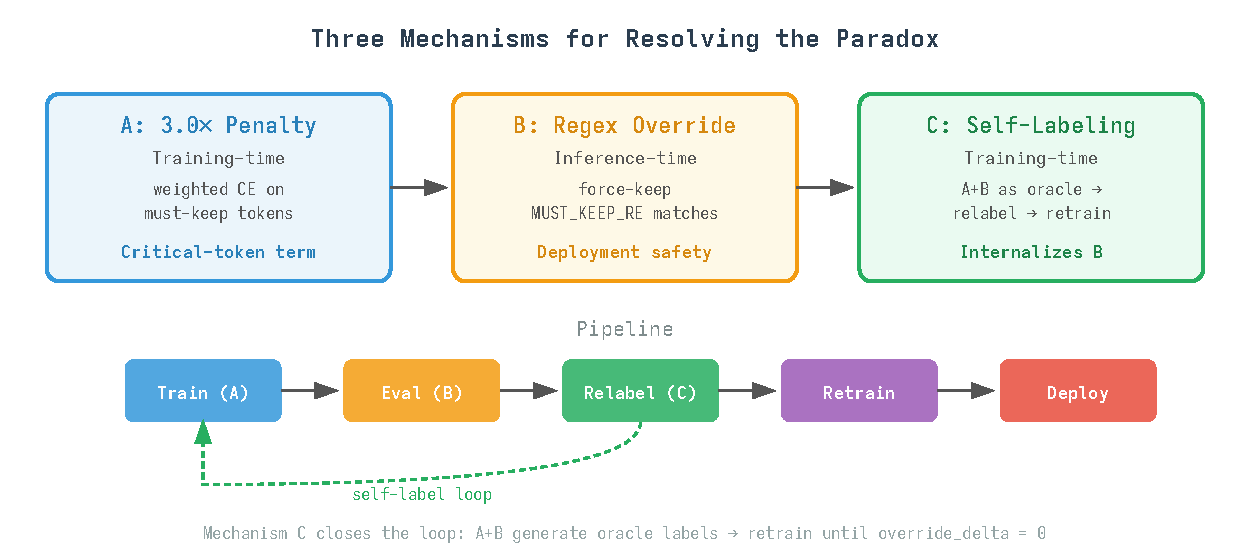
\includegraphics[width=0.85\textwidth]{fig-mechanisms.pdf}
  \caption{Three mechanisms for resolving the Voting Ensemble Paradox.
  Mechanism~A (training-time $3.0\times$ penalty) reduces false evictions.
  Mechanism~B (inference-time regex override) provides a deterministic safety
  net. Mechanism~C (self-labeling loop) closes the training loop by using A+B
  as an oracle to relabel and retrain, internalizing B until
  $\mathit{override\_delta}{=}0$.}
  \label{fig:mechanisms}
\end{figure}

\paragraph{Production pathway: C3 self-distillation.} The self-labeling loop
converged at v4/v5, but the production model v8 uses a stronger oracle: a
\textbf{Qwen2.5-7B-Instruct} teacher that labels which tokens to keep on
\emph{real agent tool outputs} (bash output, file reads, search results, JSON
tool responses, error traces). This is \emph{C3 self-distillation}:
\textbf{C}ollect real tool outputs from production traffic,
\textbf{C}urate them with the Qwen teacher's keep/drop labels, and
\textbf{C}ompress the result into the fast ModernBERT student. The training
set is 97 Qwen-labeled pairs + 200 generic multi-domain pairs (33\% C3
ratio), fine-tuned from v2-base for 3 epochs. Qwen teacher labels beat
self-labels by $+0.012$ heretic ($0.955$ vs $0.943$ on the 32-prompt set),
making v8 the production recommendation with agent
$\mathit{mk\_in\_ref}{=}1.000$ under the override.

\subsection{Training procedure}
\label{sec:train}

We freeze the base ModernBERT encoder weights (preserving pretrained syntactic
and semantic representations) and apply LoRA adapters to the last 4 of 22
transformer layers, plus retrain both task heads from scratch. Total trainable
parameters: ${\sim}2$M out of 149M.

\begin{itemize}
  \item \textbf{LoRA config:} $r{=}16$, $\alpha{=}32$, target modules
        \texttt{query}, \texttt{key}, \texttt{value},
        \texttt{layers\_to\_transform=\{18,19,20,21\}} (last 4 of 22).
  \item \textbf{Rationale:} lower layers encode syntactic structure and basic
        semantics---already correct. Higher layers encode task-specific
        salience: what is ``important'' for the current task. We shift that
        prior (``\texttt{SIGILL} is more salient than the'') without rewiring
        grammar.
  \item \textbf{Loss:} $\mathcal{L} = \mathcal{L}_{\mathrm{token}} + 0.3
        \cdot \mathcal{L}_{\mathrm{span}}$, where
        $\mathcal{L}_{\mathrm{token}}$ is the $3.0\times$-weighted
        cross-entropy (Mechanism~A) and $\mathcal{L}_{\mathrm{span}}$ is BCE
        between the span-head output and the keep mask.
  \item \textbf{Schedule:} 3 epochs, AdamW, learning rate $2\mathrm{e}{-4}$,
        batch size 16. The correctable-loop invariant halts at 3 epochs;
        v3.3 showed that near-memorization (loss $0.0007$) does not improve
        the heretic metric.
  \item \textbf{Hardware:} vast.ai RTX~4090, ${\sim}15$--25
        minutes per run.
  \item \textbf{Export:} fp32 ONNX, pushed to HuggingFace Hub
        (\texttt{PeetPedro/kompress-v*}).
  \item \textbf{v8 specifics:} 97 Qwen2.5-7B-labeled C3 pairs + 200 generic
        multi-domain pairs (33\% C3 ratio), fine-tuned from
        \texttt{kompress-v2-base}, loss $0.490\to0.431$.
\end{itemize}
